\documentclass[1p]{elsarticle_modified}
%\bibliographystyle{elsarticle-num}

%\usepackage[colorlinks]{hyperref}
%\usepackage{abbrmath_seonhwa} %\Abb, \Ascr, \Acal ,\Abf, \Afrak
\usepackage{amsfonts}
\usepackage{amssymb}
\usepackage{amsmath}
\usepackage{amsthm}
\usepackage{scalefnt}
\usepackage{amsbsy}
\usepackage{kotex}
\usepackage{caption}
\usepackage{subfig}
\usepackage{color}
\usepackage{graphicx}
\usepackage{xcolor} %% white, black, red, green, blue, cyan, magenta, yellow
\usepackage{float}
\usepackage{setspace}
\usepackage{hyperref}

\usepackage{tikz}
\usetikzlibrary{arrows}

\usepackage{multirow}
\usepackage{array} % fixed length table
\usepackage{hhline}

%%%%%%%%%%%%%%%%%%%%%
\makeatletter
\renewcommand*\env@matrix[1][\arraystretch]{%
	\edef\arraystretch{#1}%
	\hskip -\arraycolsep
	\let\@ifnextchar\new@ifnextchar
	\array{*\c@MaxMatrixCols c}}
\makeatother %https://tex.stackexchange.com/questions/14071/how-can-i-increase-the-line-spacing-in-a-matrix
%%%%%%%%%%%%%%%

\usepackage[normalem]{ulem}

\newcommand{\msout}[1]{\ifmmode\text{\sout{\ensuremath{#1}}}\else\sout{#1}\fi}
%SOURCE: \msout is \stkout macro in https://tex.stackexchange.com/questions/20609/strikeout-in-math-mode

\newcommand{\cancel}[1]{
	\ifmmode
	{\color{red}\msout{#1}}
	\else
	{\color{red}\sout{#1}}
	\fi
}

\newcommand{\add}[1]{
	{\color{blue}\uwave{#1}}
}

\newcommand{\replace}[2]{
	\ifmmode
	{\color{red}\msout{#1}}{\color{blue}\uwave{#2}}
	\else
	{\color{red}\sout{#1}}{\color{blue}\uwave{#2}}
	\fi
}

\newcommand{\Sol}{\mathcal{S}} %segment
\newcommand{\D}{D} %diagram
\newcommand{\A}{\mathcal{A}} %arc


%%%%%%%%%%%%%%%%%%%%%%%%%%%%%5 test

\def\sl{\operatorname{\textup{SL}}(2,\Cbb)}
\def\psl{\operatorname{\textup{PSL}}(2,\Cbb)}
\def\quan{\mkern 1mu \triangleright \mkern 1mu}

\theoremstyle{definition}
\newtheorem{thm}{Theorem}[section]
\newtheorem{prop}[thm]{Proposition}
\newtheorem{lem}[thm]{Lemma}
\newtheorem{ques}[thm]{Question}
\newtheorem{cor}[thm]{Corollary}
\newtheorem{defn}[thm]{Definition}
\newtheorem{exam}[thm]{Example}
\newtheorem{rmk}[thm]{Remark}
\newtheorem{alg}[thm]{Algorithm}

\newcommand{\I}{\sqrt{-1}}
\begin{document}

%\begin{frontmatter}
%
%\title{Boundary parabolic representations of knots up to 8 crossings}
%
%%% Group authors per affiliation:
%\author{Yunhi Cho} 
%\address{Department of Mathematics, University of Seoul, Seoul, Korea}
%\ead{yhcho@uos.ac.kr}
%
%
%\author{Seonhwa Kim} %\fnref{s_kim}}
%\address{Center for Geometry and Physics, Institute for Basic Science, Pohang, 37673, Korea}
%\ead{ryeona17@ibs.re.kr}
%
%\author{Hyuk Kim}
%\address{Department of Mathematical Sciences, Seoul National University, Seoul 08826, Korea}
%\ead{hyukkim@snu.ac.kr}
%
%\author{Seokbeom Yoon}
%\address{Department of Mathematical Sciences, Seoul National University, Seoul, 08826,  Korea}
%\ead{sbyoon15@snu.ac.kr}
%
%\begin{abstract}
%We find all boundary parabolic representation of knots up to 8 crossings.
%
%\end{abstract}
%\begin{keyword}
%    \MSC[2010] 57M25 
%\end{keyword}
%
%\end{frontmatter}

%\linenumbers
%\tableofcontents
%
\newcommand\colored[1]{\textcolor{white}{\rule[-0.35ex]{0.8em}{1.4ex}}\kern-0.8em\color{red} #1}%
%\newcommand\colored[1]{\textcolor{white}{ #1}\kern-2.17ex	\textcolor{white}{ #1}\kern-1.81ex	\textcolor{white}{ #1}\kern-2.15ex\color{red}#1	}

{\Large $\underline{12n_{0573}~(K12n_{0573})}$}

\setlength{\tabcolsep}{10pt}
\renewcommand{\arraystretch}{1.6}
\vspace{1cm}\begin{tabular}{m{100pt}>{\centering\arraybackslash}m{274pt}}
\multirow{5}{120pt}{
	\centering
	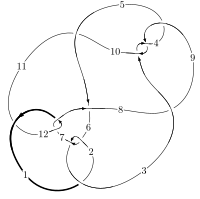
\includegraphics[width=112pt]{../../../GIT/diagram.site/Diagrams/png/2662_12n_0573.png}\\
\ \ \ A knot diagram\footnotemark}&
\allowdisplaybreaks
\textbf{Linearized knot diagam} \\
\cline{2-2}
 &
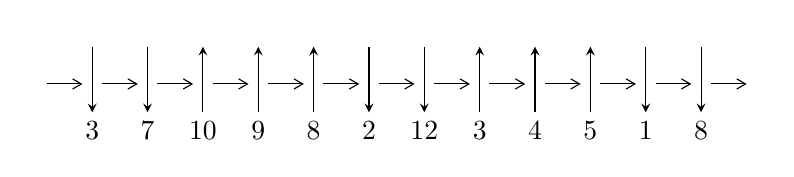
\begin{tikzpicture}[x=20pt, y=17pt]
	% nodes
	\node (C0) at (0, 0) {};
	\node (C1) at (1, 0) {};
	\node (C1U) at (1, +1) {};
	\node (C1D) at (1, -1) {3};

	\node (C2) at (2, 0) {};
	\node (C2U) at (2, +1) {};
	\node (C2D) at (2, -1) {7};

	\node (C3) at (3, 0) {};
	\node (C3U) at (3, +1) {};
	\node (C3D) at (3, -1) {10};

	\node (C4) at (4, 0) {};
	\node (C4U) at (4, +1) {};
	\node (C4D) at (4, -1) {9};

	\node (C5) at (5, 0) {};
	\node (C5U) at (5, +1) {};
	\node (C5D) at (5, -1) {8};

	\node (C6) at (6, 0) {};
	\node (C6U) at (6, +1) {};
	\node (C6D) at (6, -1) {2};

	\node (C7) at (7, 0) {};
	\node (C7U) at (7, +1) {};
	\node (C7D) at (7, -1) {12};

	\node (C8) at (8, 0) {};
	\node (C8U) at (8, +1) {};
	\node (C8D) at (8, -1) {3};

	\node (C9) at (9, 0) {};
	\node (C9U) at (9, +1) {};
	\node (C9D) at (9, -1) {4};

	\node (C10) at (10, 0) {};
	\node (C10U) at (10, +1) {};
	\node (C10D) at (10, -1) {5};

	\node (C11) at (11, 0) {};
	\node (C11U) at (11, +1) {};
	\node (C11D) at (11, -1) {1};

	\node (C12) at (12, 0) {};
	\node (C12U) at (12, +1) {};
	\node (C12D) at (12, -1) {8};
	\node (C13) at (13, 0) {};

	% arrows
	\draw[->,>={angle 60}]
	(C0) edge (C1) (C1) edge (C2) (C2) edge (C3) (C3) edge (C4) (C4) edge (C5) (C5) edge (C6) (C6) edge (C7) (C7) edge (C8) (C8) edge (C9) (C9) edge (C10) (C10) edge (C11) (C11) edge (C12) (C12) edge (C13) ;	\draw[->,>=stealth]
	(C1U) edge (C1D) (C2U) edge (C2D) (C3D) edge (C3U) (C4D) edge (C4U) (C5D) edge (C5U) (C6U) edge (C6D) (C7U) edge (C7D) (C8D) edge (C8U) (C9D) edge (C9U) (C10D) edge (C10U) (C11U) edge (C11D) (C12U) edge (C12D) ;
	\end{tikzpicture} \\
\hhline{~~} \\& 
\textbf{Solving Sequence} \\ \cline{2-2} 
 &
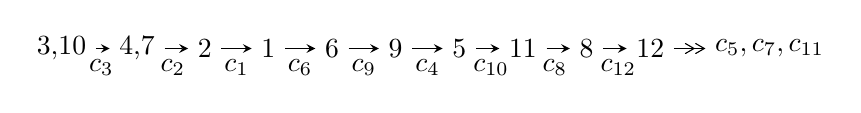
\begin{tikzpicture}[x=23pt, y=7pt]
	% node
	\node (A0) at (-1/8, 0) {3,10};
	\node (A1) at (17/16, 0) {4,7};
	\node (A2) at (17/8, 0) {2};
	\node (A3) at (25/8, 0) {1};
	\node (A4) at (33/8, 0) {6};
	\node (A5) at (41/8, 0) {9};
	\node (A6) at (49/8, 0) {5};
	\node (A7) at (57/8, 0) {11};
	\node (A8) at (65/8, 0) {8};
	\node (A9) at (73/8, 0) {12};
	\node (C1) at (1/2, -1) {$c_{3}$};
	\node (C2) at (13/8, -1) {$c_{2}$};
	\node (C3) at (21/8, -1) {$c_{1}$};
	\node (C4) at (29/8, -1) {$c_{6}$};
	\node (C5) at (37/8, -1) {$c_{9}$};
	\node (C6) at (45/8, -1) {$c_{4}$};
	\node (C7) at (53/8, -1) {$c_{10}$};
	\node (C8) at (61/8, -1) {$c_{8}$};
	\node (C9) at (69/8, -1) {$c_{12}$};
	\node (A10) at (11, 0) {$c_{5},c_{7},c_{11}$};

	% edge
	\draw[->,>=stealth]	
	(A0) edge (A1) (A1) edge (A2) (A2) edge (A3) (A3) edge (A4) (A4) edge (A5) (A5) edge (A6) (A6) edge (A7) (A7) edge (A8) (A8) edge (A9) ;
	\draw[->>,>={angle 60}]	
	(A9) edge (A10);
\end{tikzpicture} \\ 

\end{tabular} \\

\footnotetext{
The image of knot diagram is generated by the software ``\textbf{Draw programme}" developed by Andrew Bartholomew(\url{http://www.layer8.co.uk/maths/draw/index.htm\#Running-draw}), where we modified some parts for our purpose(\url{https://github.com/CATsTAILs/LinksPainter}).
}\phantom \\ \newline 
\centering \textbf{Ideals for irreducible components\footnotemark of $X_{\text{par}}$} 
 
\begin{align*}
I^u_{1}&=\langle 
u^{16}- u^{15}+\cdots+b+1,\;- u^{18}+3 u^{17}+\cdots+2 a-6,\;u^{19}-3 u^{18}+\cdots+6 u-2\rangle \\
I^u_{2}&=\langle 
24 u^8 a+207 u^8+\cdots+31 a-237,\\
\phantom{I^u_{2}}&\phantom{= \langle  }2 u^8 a+u^8+6 u^6 a+5 u^6+6 u^4 a- u^5+8 u^4-2 u^2 a-2 u^3+a^2+a u+2 u^2-4 a-3,\\
\phantom{I^u_{2}}&\phantom{= \langle  }u^9+u^8+4 u^7+3 u^6+5 u^5+3 u^4-3 u-1\rangle \\
I^u_{3}&=\langle 
b-1,\;-2 u^3-3 u^2+3 a-3 u-3,\;u^4+3 u^2+3\rangle \\
I^u_{4}&=\langle 
b+1,\;- u^2+a- u-1,\;u^4+u^2-1\rangle \\
\\
I^v_{1}&=\langle 
a,\;b-1,\;v+1\rangle \\
\end{align*}
\raggedright * 5 irreducible components of $\dim_{\mathbb{C}}=0$, with total 46 representations.\\
\footnotetext{All coefficients of polynomials are rational numbers. But the coefficients are sometimes approximated in decimal forms when there is not enough margin.}
\newpage
\renewcommand{\arraystretch}{1}
\centering \section*{I. $I^u_{1}= \langle u^{16}- u^{15}+\cdots+b+1,\;- u^{18}+3 u^{17}+\cdots+2 a-6,\;u^{19}-3 u^{18}+\cdots+6 u-2 \rangle$}
\flushleft \textbf{(i) Arc colorings}\\
\begin{tabular}{m{7pt} m{180pt} m{7pt} m{180pt} }
\flushright $a_{3}=$&$\begin{pmatrix}1\\0\end{pmatrix}$ \\
\flushright $a_{10}=$&$\begin{pmatrix}0\\u\end{pmatrix}$ \\
\flushright $a_{4}=$&$\begin{pmatrix}1\\- u^2\end{pmatrix}$ \\
\flushright $a_{7}=$&$\begin{pmatrix}\frac{1}{2} u^{18}-\frac{3}{2} u^{17}+\cdots-\frac{7}{2} u+3\\- u^{16}+u^{15}+\cdots+u-1\end{pmatrix}$ \\
\flushright $a_{2}=$&$\begin{pmatrix}-\frac{3}{2} u^{18}+\frac{5}{2} u^{17}+\cdots+\frac{7}{2} u-1\\u^{18}-2 u^{17}+\cdots-2 u+1\end{pmatrix}$ \\
\flushright $a_{1}=$&$\begin{pmatrix}-\frac{1}{2} u^{18}+\frac{1}{2} u^{17}+\cdots-\frac{5}{2} u^2+\frac{3}{2} u\\u^{18}-2 u^{17}+\cdots-2 u+1\end{pmatrix}$ \\
\flushright $a_{6}=$&$\begin{pmatrix}- u^{10}-5 u^8-8 u^6-3 u^4+3 u^2+1\\u^{10}+4 u^8+5 u^6-3 u^2\end{pmatrix}$ \\
\flushright $a_{9}=$&$\begin{pmatrix}- u\\u^3+u\end{pmatrix}$ \\
\flushright $a_{5}=$&$\begin{pmatrix}u^2+1\\- u^4-2 u^2\end{pmatrix}$ \\
\flushright $a_{11}=$&$\begin{pmatrix}u^5+2 u^3+u\\- u^7-3 u^5-2 u^3+u\end{pmatrix}$ \\
\flushright $a_{8}=$&$\begin{pmatrix}- u^3-2 u\\u^3+u\end{pmatrix}$ \\
\flushright $a_{12}=$&$\begin{pmatrix}\frac{3}{2} u^{18}-\frac{5}{2} u^{17}+\cdots-\frac{5}{2} u+2\\- u^{18}+2 u^{17}+\cdots+3 u-1\end{pmatrix}$\\&\end{tabular}
\flushleft \textbf{(ii) Obstruction class $= -1$}\\~\\
\flushleft \textbf{(iii) Cusp Shapes $= -2 u^{17}+6 u^{16}-22 u^{15}+44 u^{14}-88 u^{13}+124 u^{12}-164 u^{11}+158 u^{10}-134 u^9+68 u^8-10 u^7-26 u^6+42 u^5-14 u^4+2 u^3+18 u^2-20 u+8$}\\~\\
\newpage\renewcommand{\arraystretch}{1}
\flushleft \textbf{(iv) u-Polynomials at the component}\newline \\
\begin{tabular}{m{50pt}|m{274pt}}
Crossings & \hspace{64pt}u-Polynomials at each crossing \\
\hline $$\begin{aligned}c_{1},c_{11}\end{aligned}$$&$\begin{aligned}
&u^{19}+3 u^{18}+\cdots+7 u+1
\end{aligned}$\\
\hline $$\begin{aligned}c_{2},c_{6},c_{7}\\c_{12}\end{aligned}$$&$\begin{aligned}
&u^{19}- u^{18}+\cdots- u-1
\end{aligned}$\\
\hline $$\begin{aligned}c_{3},c_{4},c_{9}\end{aligned}$$&$\begin{aligned}
&u^{19}-3 u^{18}+\cdots+6 u-2
\end{aligned}$\\
\hline $$\begin{aligned}c_{5}\end{aligned}$$&$\begin{aligned}
&u^{19}+21 u^{18}+\cdots+2406 u+562
\end{aligned}$\\
\hline $$\begin{aligned}c_{8},c_{10}\end{aligned}$$&$\begin{aligned}
&u^{19}+3 u^{18}+\cdots+14 u-10
\end{aligned}$\\
\hline
\end{tabular}\\~\\
\newpage\renewcommand{\arraystretch}{1}
\flushleft \textbf{(v) Riley Polynomials at the component}\newline \\
\begin{tabular}{m{50pt}|m{274pt}}
Crossings & \hspace{64pt}Riley Polynomials at each crossing \\
\hline $$\begin{aligned}c_{1},c_{11}\end{aligned}$$&$\begin{aligned}
&y^{19}+37 y^{18}+\cdots+7 y-1
\end{aligned}$\\
\hline $$\begin{aligned}c_{2},c_{6},c_{7}\\c_{12}\end{aligned}$$&$\begin{aligned}
&y^{19}-3 y^{18}+\cdots+7 y-1
\end{aligned}$\\
\hline $$\begin{aligned}c_{3},c_{4},c_{9}\end{aligned}$$&$\begin{aligned}
&y^{19}+15 y^{18}+\cdots-16 y-4
\end{aligned}$\\
\hline $$\begin{aligned}c_{5}\end{aligned}$$&$\begin{aligned}
&y^{19}-45 y^{18}+\cdots-2597328 y-315844
\end{aligned}$\\
\hline $$\begin{aligned}c_{8},c_{10}\end{aligned}$$&$\begin{aligned}
&y^{19}-21 y^{18}+\cdots-384 y-100
\end{aligned}$\\
\hline
\end{tabular}\\~\\
\newpage\flushleft \textbf{(vi) Complex Volumes and Cusp Shapes}
$$\begin{array}{c|c|c}  
\text{Solutions to }I^u_{1}& \I (\text{vol} + \sqrt{-1}CS) & \text{Cusp shape}\\
 \hline 
\begin{aligned}
u &= -0.304317 + 0.981930 I \\
a &= -0.73640 + 1.23198 I \\
b &= \phantom{-}0.534624 - 0.866654 I\end{aligned}
 & \phantom{-}0.619243 + 0.825287 I & \phantom{-}1.58746 - 1.31207 I \\ \hline\begin{aligned}
u &= -0.304317 - 0.981930 I \\
a &= -0.73640 - 1.23198 I \\
b &= \phantom{-}0.534624 + 0.866654 I\end{aligned}
 & \phantom{-}0.619243 - 0.825287 I & \phantom{-}1.58746 + 1.31207 I \\ \hline\begin{aligned}
u &= \phantom{-}0.929404 + 0.054061 I \\
a &= -1.85707 + 2.86205 I \\
b &= \phantom{-}1.16834 - 0.97470 I\end{aligned}
 & \phantom{-}11.9496 + 7.7615 I & \phantom{-}2.99197 - 4.29762 I \\ \hline\begin{aligned}
u &= \phantom{-}0.929404 - 0.054061 I \\
a &= -1.85707 - 2.86205 I \\
b &= \phantom{-}1.16834 + 0.97470 I\end{aligned}
 & \phantom{-}11.9496 - 7.7615 I & \phantom{-}2.99197 + 4.29762 I \\ \hline\begin{aligned}
u &= \phantom{-}0.744027\phantom{ +0.000000I} \\
a &= \phantom{-}0.660757\phantom{ +0.000000I} \\
b &= -0.577590\phantom{ +0.000000I}\end{aligned}
 & \phantom{-}2.21133\phantom{ +0.000000I} & \phantom{-}4.57840\phantom{ +0.000000I} \\ \hline\begin{aligned}
u &= -0.689684 + 0.229296 I \\
a &= \phantom{-}0.50396 + 2.44275 I \\
b &= -0.768036 - 0.810356 I\end{aligned}
 & \phantom{-}2.79530 - 4.62119 I & \phantom{-}3.18170 + 6.56238 I \\ \hline\begin{aligned}
u &= -0.689684 - 0.229296 I \\
a &= \phantom{-}0.50396 - 2.44275 I \\
b &= -0.768036 + 0.810356 I\end{aligned}
 & \phantom{-}2.79530 + 4.62119 I & \phantom{-}3.18170 - 6.56238 I \\ \hline\begin{aligned}
u &= \phantom{-}0.315935 + 1.282700 I \\
a &= -0.038879 + 0.454563 I \\
b &= \phantom{-}0.606078 + 0.079526 I\end{aligned}
 & -1.79110 + 3.82280 I & -0.01419 - 2.05902 I \\ \hline\begin{aligned}
u &= \phantom{-}0.315935 - 1.282700 I \\
a &= -0.038879 - 0.454563 I \\
b &= \phantom{-}0.606078 - 0.079526 I\end{aligned}
 & -1.79110 - 3.82280 I & -0.01419 + 2.05902 I \\ \hline\begin{aligned}
u &= \phantom{-}0.473566 + 1.246700 I \\
a &= \phantom{-}1.69399 + 1.30200 I \\
b &= -1.12434 - 1.01004 I\end{aligned}
 & \phantom{-}8.26951 - 2.76755 I & \phantom{-}0.165642 + 1.152780 I\\
 \hline 
 \end{array}$$\newpage$$\begin{array}{c|c|c}  
\text{Solutions to }I^u_{1}& \I (\text{vol} + \sqrt{-1}CS) & \text{Cusp shape}\\
 \hline 
\begin{aligned}
u &= \phantom{-}0.473566 - 1.246700 I \\
a &= \phantom{-}1.69399 - 1.30200 I \\
b &= -1.12434 + 1.01004 I\end{aligned}
 & \phantom{-}8.26951 + 2.76755 I & \phantom{-}0.165642 - 1.152780 I \\ \hline\begin{aligned}
u &= -0.000906 + 1.344200 I \\
a &= -0.628189 - 0.110568 I \\
b &= -0.631711 + 0.410114 I\end{aligned}
 & -5.42437 + 1.46948 I & -4.90135 - 4.71907 I \\ \hline\begin{aligned}
u &= -0.000906 - 1.344200 I \\
a &= -0.628189 + 0.110568 I \\
b &= -0.631711 - 0.410114 I\end{aligned}
 & -5.42437 - 1.46948 I & -4.90135 + 4.71907 I \\ \hline\begin{aligned}
u &= -0.250312 + 1.349130 I \\
a &= \phantom{-}0.61482 - 1.58026 I \\
b &= \phantom{-}0.876351 + 0.702623 I\end{aligned}
 & -2.18836 - 7.94720 I & -2.76731 + 8.17106 I \\ \hline\begin{aligned}
u &= -0.250312 - 1.349130 I \\
a &= \phantom{-}0.61482 + 1.58026 I \\
b &= \phantom{-}0.876351 - 0.702623 I\end{aligned}
 & -2.18836 + 7.94720 I & -2.76731 - 8.17106 I \\ \hline\begin{aligned}
u &= \phantom{-}0.435648 + 1.328780 I \\
a &= \phantom{-}0.25932 - 2.69648 I \\
b &= -1.19156 + 0.93252 I\end{aligned}
 & \phantom{-}7.6280 + 12.6384 I & -0.71689 - 6.92034 I \\ \hline\begin{aligned}
u &= \phantom{-}0.435648 - 1.328780 I \\
a &= \phantom{-}0.25932 + 2.69648 I \\
b &= -1.19156 - 0.93252 I\end{aligned}
 & \phantom{-}7.6280 - 12.6384 I & -0.71689 + 6.92034 I \\ \hline\begin{aligned}
u &= \phantom{-}0.218652 + 0.470395 I \\
a &= \phantom{-}0.358071 + 0.971620 I \\
b &= \phantom{-}0.319050 - 0.558488 I\end{aligned}
 & \phantom{-}0.065587 + 1.130710 I & \phantom{-}1.18374 - 5.82659 I \\ \hline\begin{aligned}
u &= \phantom{-}0.218652 - 0.470395 I \\
a &= \phantom{-}0.358071 - 0.971620 I \\
b &= \phantom{-}0.319050 + 0.558488 I\end{aligned}
 & \phantom{-}0.065587 - 1.130710 I & \phantom{-}1.18374 + 5.82659 I\\
 \hline 
 \end{array}$$\newpage\newpage\renewcommand{\arraystretch}{1}
\centering \section*{II. $I^u_{2}= \langle 24 u^8 a+207 u^8+\cdots+31 a-237,\;2 u^8 a+u^8+\cdots-4 a-3,\;u^9+u^8+4 u^7+3 u^6+5 u^5+3 u^4-3 u-1 \rangle$}
\flushleft \textbf{(i) Arc colorings}\\
\begin{tabular}{m{7pt} m{180pt} m{7pt} m{180pt} }
\flushright $a_{3}=$&$\begin{pmatrix}1\\0\end{pmatrix}$ \\
\flushright $a_{10}=$&$\begin{pmatrix}0\\u\end{pmatrix}$ \\
\flushright $a_{4}=$&$\begin{pmatrix}1\\- u^2\end{pmatrix}$ \\
\flushright $a_{7}=$&$\begin{pmatrix}a\\-0.0892193 a u^{8}-0.769517 u^{8}+\cdots-0.115242 a+0.881041\end{pmatrix}$ \\
\flushright $a_{2}=$&$\begin{pmatrix}-0.769517 a u^{8}-0.762082 u^{8}+\cdots+0.881041 a+1.97398\\0.163569 a u^{8}-0.0892193 u^{8}+\cdots+0.0446097 a-1.11524\end{pmatrix}$ \\
\flushright $a_{1}=$&$\begin{pmatrix}-0.605948 a u^{8}-0.851301 u^{8}+\cdots+0.925651 a+0.858736\\0.163569 a u^{8}-0.0892193 u^{8}+\cdots+0.0446097 a-1.11524\end{pmatrix}$ \\
\flushright $a_{6}=$&$\begin{pmatrix}-2 u^8- u^7-6 u^6-2 u^5-6 u^4+2 u+2\\u^8+u^7+3 u^6+2 u^5+3 u^4-2 u-1\end{pmatrix}$ \\
\flushright $a_{9}=$&$\begin{pmatrix}- u\\u^3+u\end{pmatrix}$ \\
\flushright $a_{5}=$&$\begin{pmatrix}u^2+1\\- u^4-2 u^2\end{pmatrix}$ \\
\flushright $a_{11}=$&$\begin{pmatrix}u^5+2 u^3+u\\- u^7-3 u^5-2 u^3+u\end{pmatrix}$ \\
\flushright $a_{8}=$&$\begin{pmatrix}- u^3-2 u\\u^3+u\end{pmatrix}$ \\
\flushright $a_{12}=$&$\begin{pmatrix}-0.769517 a u^{8}-0.762082 u^{8}+\cdots+0.881041 a-0.0260223\\-1\end{pmatrix}$\\&\end{tabular}
\flushleft \textbf{(ii) Obstruction class $= -1$}\\~\\
\flushleft \textbf{(iii) Cusp Shapes $= -4 u^8-4 u^7-12 u^6-8 u^5-8 u^4-4 u^3+8 u^2+4 u+6$}\\~\\
\newpage\renewcommand{\arraystretch}{1}
\flushleft \textbf{(iv) u-Polynomials at the component}\newline \\
\begin{tabular}{m{50pt}|m{274pt}}
Crossings & \hspace{64pt}u-Polynomials at each crossing \\
\hline $$\begin{aligned}c_{1},c_{11}\end{aligned}$$&$\begin{aligned}
&u^{18}+5 u^{17}+\cdots+4 u+1
\end{aligned}$\\
\hline $$\begin{aligned}c_{2},c_{6},c_{7}\\c_{12}\end{aligned}$$&$\begin{aligned}
&u^{18}- u^{17}+\cdots+2 u-1
\end{aligned}$\\
\hline $$\begin{aligned}c_{3},c_{4},c_{9}\end{aligned}$$&$\begin{aligned}
&(u^9+u^8+4 u^7+3 u^6+5 u^5+3 u^4-3 u-1)^2
\end{aligned}$\\
\hline $$\begin{aligned}c_{5}\end{aligned}$$&$\begin{aligned}
&(u^9-7 u^8+6 u^7+37 u^6-21 u^5-89 u^4-66 u^3-54 u^2-39 u-7)^2
\end{aligned}$\\
\hline $$\begin{aligned}c_{8},c_{10}\end{aligned}$$&$\begin{aligned}
&(u^9- u^8-6 u^7+5 u^6+11 u^5-7 u^4-6 u^3+4 u^2- u-1)^2
\end{aligned}$\\
\hline
\end{tabular}\\~\\
\newpage\renewcommand{\arraystretch}{1}
\flushleft \textbf{(v) Riley Polynomials at the component}\newline \\
\begin{tabular}{m{50pt}|m{274pt}}
Crossings & \hspace{64pt}Riley Polynomials at each crossing \\
\hline $$\begin{aligned}c_{1},c_{11}\end{aligned}$$&$\begin{aligned}
&y^{18}+15 y^{17}+\cdots-52 y+1
\end{aligned}$\\
\hline $$\begin{aligned}c_{2},c_{6},c_{7}\\c_{12}\end{aligned}$$&$\begin{aligned}
&y^{18}-5 y^{17}+\cdots-4 y+1
\end{aligned}$\\
\hline $$\begin{aligned}c_{3},c_{4},c_{9}\end{aligned}$$&$\begin{aligned}
&(y^9+7 y^8+20 y^7+25 y^6+y^5-31 y^4-24 y^3+6 y^2+9 y-1)^2
\end{aligned}$\\
\hline $$\begin{aligned}c_{5}\end{aligned}$$&$\begin{aligned}
&(y^9-37 y^8+\cdots+765 y-49)^{2}
\end{aligned}$\\
\hline $$\begin{aligned}c_{8},c_{10}\end{aligned}$$&$\begin{aligned}
&(y^9-13 y^8+68 y^7-183 y^6+269 y^5-211 y^4+80 y^3-18 y^2+9 y-1)^{2}
\end{aligned}$\\
\hline
\end{tabular}\\~\\
\newpage\flushleft \textbf{(vi) Complex Volumes and Cusp Shapes}
$$\begin{array}{c|c|c}  
\text{Solutions to }I^u_{2}& \I (\text{vol} + \sqrt{-1}CS) & \text{Cusp shape}\\
 \hline 
\begin{aligned}
u &= -0.940385\phantom{ +0.000000I} \\
a &= -1.67785 + 2.94580 I \\
b &= \phantom{-}0.88600 - 1.16403 I\end{aligned}
 & \phantom{-}12.9028\phantom{ +0.000000I} & \phantom{-}4.12280\phantom{ +0.000000I} \\ \hline\begin{aligned}
u &= -0.940385\phantom{ +0.000000I} \\
a &= -1.67785 - 2.94580 I \\
b &= \phantom{-}0.88600 + 1.16403 I\end{aligned}
 & \phantom{-}12.9028\phantom{ +0.000000I} & \phantom{-}4.12280\phantom{ +0.000000I} \\ \hline\begin{aligned}
u &= -0.105528 + 1.193370 I \\
a &= -0.612327 - 0.108328 I \\
b &= -1.214940 + 0.117733 I\end{aligned}
 & -6.13776 - 1.55423 I & -5.05960 + 4.30527 I \\ \hline\begin{aligned}
u &= -0.105528 + 1.193370 I \\
a &= -0.85424 - 2.40749 I \\
b &= \phantom{-}0.870781 + 0.348555 I\end{aligned}
 & -6.13776 - 1.55423 I & -5.05960 + 4.30527 I \\ \hline\begin{aligned}
u &= -0.105528 - 1.193370 I \\
a &= -0.612327 + 0.108328 I \\
b &= -1.214940 - 0.117733 I\end{aligned}
 & -6.13776 + 1.55423 I & -5.05960 - 4.30527 I \\ \hline\begin{aligned}
u &= -0.105528 - 1.193370 I \\
a &= -0.85424 + 2.40749 I \\
b &= \phantom{-}0.870781 - 0.348555 I\end{aligned}
 & -6.13776 + 1.55423 I & -5.05960 - 4.30527 I \\ \hline\begin{aligned}
u &= \phantom{-}0.743788\phantom{ +0.000000I} \\
a &= \phantom{-}0.661558 + 0.082738 I \\
b &= -0.577633 - 0.031295 I\end{aligned}
 & \phantom{-}2.21133\phantom{ +0.000000I} & \phantom{-}4.57530\phantom{ +0.000000I} \\ \hline\begin{aligned}
u &= \phantom{-}0.743788\phantom{ +0.000000I} \\
a &= \phantom{-}0.661558 - 0.082738 I \\
b &= -0.577633 + 0.031295 I\end{aligned}
 & \phantom{-}2.21133\phantom{ +0.000000I} & \phantom{-}4.57530\phantom{ +0.000000I} \\ \hline\begin{aligned}
u &= \phantom{-}0.328404 + 1.225450 I \\
a &= \phantom{-}0.279234 - 0.828501 I \\
b &= \phantom{-}0.067133 + 0.481523 I\end{aligned}
 & -1.53180 + 3.86354 I & \phantom{-}0.03791 - 4.00946 I \\ \hline\begin{aligned}
u &= \phantom{-}0.328404 + 1.225450 I \\
a &= -0.455774 + 1.279350 I \\
b &= \phantom{-}1.048570 - 0.263166 I\end{aligned}
 & -1.53180 + 3.86354 I & \phantom{-}0.03791 - 4.00946 I\\
 \hline 
 \end{array}$$\newpage$$\begin{array}{c|c|c}  
\text{Solutions to }I^u_{2}& \I (\text{vol} + \sqrt{-1}CS) & \text{Cusp shape}\\
 \hline 
\begin{aligned}
u &= \phantom{-}0.328404 - 1.225450 I \\
a &= \phantom{-}0.279234 + 0.828501 I \\
b &= \phantom{-}0.067133 - 0.481523 I\end{aligned}
 & -1.53180 - 3.86354 I & \phantom{-}0.03791 + 4.00946 I \\ \hline\begin{aligned}
u &= \phantom{-}0.328404 - 1.225450 I \\
a &= -0.455774 - 1.279350 I \\
b &= \phantom{-}1.048570 + 0.263166 I\end{aligned}
 & -1.53180 - 3.86354 I & \phantom{-}0.03791 + 4.00946 I \\ \hline\begin{aligned}
u &= -0.460882 + 1.295330 I \\
a &= \phantom{-}1.69755 - 1.44384 I \\
b &= -0.82021 + 1.17863 I\end{aligned}
 & \phantom{-}8.87899 - 4.99486 I & \phantom{-}0.86627 + 2.90812 I \\ \hline\begin{aligned}
u &= -0.460882 + 1.295330 I \\
a &= \phantom{-}0.22926 + 2.59994 I \\
b &= -0.94094 - 1.12597 I\end{aligned}
 & \phantom{-}8.87899 - 4.99486 I & \phantom{-}0.86627 + 2.90812 I \\ \hline\begin{aligned}
u &= -0.460882 - 1.295330 I \\
a &= \phantom{-}1.69755 + 1.44384 I \\
b &= -0.82021 - 1.17863 I\end{aligned}
 & \phantom{-}8.87899 + 4.99486 I & \phantom{-}0.86627 - 2.90812 I \\ \hline\begin{aligned}
u &= -0.460882 - 1.295330 I \\
a &= \phantom{-}0.22926 - 2.59994 I \\
b &= -0.94094 + 1.12597 I\end{aligned}
 & \phantom{-}8.87899 + 4.99486 I & \phantom{-}0.86627 - 2.90812 I \\ \hline\begin{aligned}
u &= -0.327390\phantom{ +0.000000I} \\
a &= -0.523848\phantom{ +0.000000I} \\
b &= \phantom{-}1.13069\phantom{ +0.000000I}\end{aligned}
 & -2.72863\phantom{ +0.000000I} & \phantom{-}5.61280\phantom{ +0.000000I} \\ \hline\begin{aligned}
u &= -0.327390\phantom{ +0.000000I} \\
a &= \phantom{-}4.98902\phantom{ +0.000000I} \\
b &= -0.768210\phantom{ +0.000000I}\end{aligned}
 & -2.72863\phantom{ +0.000000I} & \phantom{-}5.61280\phantom{ +0.000000I}\\
 \hline 
 \end{array}$$\newpage\newpage\renewcommand{\arraystretch}{1}
\centering \section*{III. $I^u_{3}= \langle b-1,\;-2 u^3-3 u^2+3 a-3 u-3,\;u^4+3 u^2+3 \rangle$}
\flushleft \textbf{(i) Arc colorings}\\
\begin{tabular}{m{7pt} m{180pt} m{7pt} m{180pt} }
\flushright $a_{3}=$&$\begin{pmatrix}1\\0\end{pmatrix}$ \\
\flushright $a_{10}=$&$\begin{pmatrix}0\\u\end{pmatrix}$ \\
\flushright $a_{4}=$&$\begin{pmatrix}1\\- u^2\end{pmatrix}$ \\
\flushright $a_{7}=$&$\begin{pmatrix}\frac{2}{3} u^3+u^2+u+1\\1\end{pmatrix}$ \\
\flushright $a_{2}=$&$\begin{pmatrix}-\frac{2}{3} u^3- u^2- u\\-1\end{pmatrix}$ \\
\flushright $a_{1}=$&$\begin{pmatrix}-\frac{2}{3} u^3- u^2- u-1\\-1\end{pmatrix}$ \\
\flushright $a_{6}=$&$\begin{pmatrix}1\\0\end{pmatrix}$ \\
\flushright $a_{9}=$&$\begin{pmatrix}- u\\u^3+u\end{pmatrix}$ \\
\flushright $a_{5}=$&$\begin{pmatrix}u^2+1\\u^2+3\end{pmatrix}$ \\
\flushright $a_{11}=$&$\begin{pmatrix}- u^3-2 u\\u^3+u\end{pmatrix}$ \\
\flushright $a_{8}=$&$\begin{pmatrix}- u^3-2 u\\u^3+u\end{pmatrix}$ \\
\flushright $a_{12}=$&$\begin{pmatrix}-\frac{5}{3} u^3- u^2-3 u-1\\u^3+u-1\end{pmatrix}$\\&\end{tabular}
\flushleft \textbf{(ii) Obstruction class $= 1$}\\~\\
\flushleft \textbf{(iii) Cusp Shapes $= -4 u^2-12$}\\~\\
\newpage\renewcommand{\arraystretch}{1}
\flushleft \textbf{(iv) u-Polynomials at the component}\newline \\
\begin{tabular}{m{50pt}|m{274pt}}
Crossings & \hspace{64pt}u-Polynomials at each crossing \\
\hline $$\begin{aligned}c_{1},c_{2},c_{7}\\c_{11}\end{aligned}$$&$\begin{aligned}
&(u-1)^4
\end{aligned}$\\
\hline $$\begin{aligned}c_{3},c_{4},c_{9}\end{aligned}$$&$\begin{aligned}
&u^4+3 u^2+3
\end{aligned}$\\
\hline $$\begin{aligned}c_{5},c_{8},c_{10}\end{aligned}$$&$\begin{aligned}
&u^4-3 u^2+3
\end{aligned}$\\
\hline $$\begin{aligned}c_{6},c_{12}\end{aligned}$$&$\begin{aligned}
&(u+1)^4
\end{aligned}$\\
\hline
\end{tabular}\\~\\
\newpage\renewcommand{\arraystretch}{1}
\flushleft \textbf{(v) Riley Polynomials at the component}\newline \\
\begin{tabular}{m{50pt}|m{274pt}}
Crossings & \hspace{64pt}Riley Polynomials at each crossing \\
\hline $$\begin{aligned}c_{1},c_{2},c_{6}\\c_{7},c_{11},c_{12}\end{aligned}$$&$\begin{aligned}
&(y-1)^4
\end{aligned}$\\
\hline $$\begin{aligned}c_{3},c_{4},c_{9}\end{aligned}$$&$\begin{aligned}
&(y^2+3 y+3)^2
\end{aligned}$\\
\hline $$\begin{aligned}c_{5},c_{8},c_{10}\end{aligned}$$&$\begin{aligned}
&(y^2-3 y+3)^2
\end{aligned}$\\
\hline
\end{tabular}\\~\\
\newpage\flushleft \textbf{(vi) Complex Volumes and Cusp Shapes}
$$\begin{array}{c|c|c}  
\text{Solutions to }I^u_{3}& \I (\text{vol} + \sqrt{-1}CS) & \text{Cusp shape}\\
 \hline 
\begin{aligned}
u &= \phantom{-}0.340625 + 1.271230 I \\
a &= -1.23394 + 1.06269 I \\
b &= \phantom{-}1.00000\phantom{ +0.000000I}\end{aligned}
 & -3.28987 + 4.05977 I & -6.00000 - 3.46410 I \\ \hline\begin{aligned}
u &= \phantom{-}0.340625 - 1.271230 I \\
a &= -1.23394 - 1.06269 I \\
b &= \phantom{-}1.00000\phantom{ +0.000000I}\end{aligned}
 & -3.28987 - 4.05977 I & -6.00000 + 3.46410 I \\ \hline\begin{aligned}
u &= -0.340625 + 1.271230 I \\
a &= \phantom{-}0.233945 - 0.669365 I \\
b &= \phantom{-}1.00000\phantom{ +0.000000I}\end{aligned}
 & -3.28987 - 4.05977 I & -6.00000 + 3.46410 I \\ \hline\begin{aligned}
u &= -0.340625 - 1.271230 I \\
a &= \phantom{-}0.233945 + 0.669365 I \\
b &= \phantom{-}1.00000\phantom{ +0.000000I}\end{aligned}
 & -3.28987 + 4.05977 I & -6.00000 - 3.46410 I\\
 \hline 
 \end{array}$$\newpage\newpage\renewcommand{\arraystretch}{1}
\centering \section*{IV. $I^u_{4}= \langle b+1,\;- u^2+a- u-1,\;u^4+u^2-1 \rangle$}
\flushleft \textbf{(i) Arc colorings}\\
\begin{tabular}{m{7pt} m{180pt} m{7pt} m{180pt} }
\flushright $a_{3}=$&$\begin{pmatrix}1\\0\end{pmatrix}$ \\
\flushright $a_{10}=$&$\begin{pmatrix}0\\u\end{pmatrix}$ \\
\flushright $a_{4}=$&$\begin{pmatrix}1\\- u^2\end{pmatrix}$ \\
\flushright $a_{7}=$&$\begin{pmatrix}u^2+u+1\\-1\end{pmatrix}$ \\
\flushright $a_{2}=$&$\begin{pmatrix}u^2+u+2\\-1\end{pmatrix}$ \\
\flushright $a_{1}=$&$\begin{pmatrix}u^2+u+1\\-1\end{pmatrix}$ \\
\flushright $a_{6}=$&$\begin{pmatrix}-1\\0\end{pmatrix}$ \\
\flushright $a_{9}=$&$\begin{pmatrix}- u\\u^3+u\end{pmatrix}$ \\
\flushright $a_{5}=$&$\begin{pmatrix}u^2+1\\- u^2-1\end{pmatrix}$ \\
\flushright $a_{11}=$&$\begin{pmatrix}u^3+2 u\\- u^3- u\end{pmatrix}$ \\
\flushright $a_{8}=$&$\begin{pmatrix}- u^3-2 u\\u^3+u\end{pmatrix}$ \\
\flushright $a_{12}=$&$\begin{pmatrix}u^3+u^2+3 u+1\\- u^3- u-1\end{pmatrix}$\\&\end{tabular}
\flushleft \textbf{(ii) Obstruction class $= 1$}\\~\\
\flushleft \textbf{(iii) Cusp Shapes $= 4 u^2-4$}\\~\\
\newpage\renewcommand{\arraystretch}{1}
\flushleft \textbf{(iv) u-Polynomials at the component}\newline \\
\begin{tabular}{m{50pt}|m{274pt}}
Crossings & \hspace{64pt}u-Polynomials at each crossing \\
\hline $$\begin{aligned}c_{1},c_{6},c_{11}\\c_{12}\end{aligned}$$&$\begin{aligned}
&(u-1)^4
\end{aligned}$\\
\hline $$\begin{aligned}c_{2},c_{7}\end{aligned}$$&$\begin{aligned}
&(u+1)^4
\end{aligned}$\\
\hline $$\begin{aligned}c_{3},c_{4},c_{9}\end{aligned}$$&$\begin{aligned}
&u^4+u^2-1
\end{aligned}$\\
\hline $$\begin{aligned}c_{5},c_{8},c_{10}\end{aligned}$$&$\begin{aligned}
&u^4- u^2-1
\end{aligned}$\\
\hline
\end{tabular}\\~\\
\newpage\renewcommand{\arraystretch}{1}
\flushleft \textbf{(v) Riley Polynomials at the component}\newline \\
\begin{tabular}{m{50pt}|m{274pt}}
Crossings & \hspace{64pt}Riley Polynomials at each crossing \\
\hline $$\begin{aligned}c_{1},c_{2},c_{6}\\c_{7},c_{11},c_{12}\end{aligned}$$&$\begin{aligned}
&(y-1)^4
\end{aligned}$\\
\hline $$\begin{aligned}c_{3},c_{4},c_{9}\end{aligned}$$&$\begin{aligned}
&(y^2+y-1)^2
\end{aligned}$\\
\hline $$\begin{aligned}c_{5},c_{8},c_{10}\end{aligned}$$&$\begin{aligned}
&(y^2- y-1)^2
\end{aligned}$\\
\hline
\end{tabular}\\~\\
\newpage\flushleft \textbf{(vi) Complex Volumes and Cusp Shapes}
$$\begin{array}{c|c|c}  
\text{Solutions to }I^u_{4}& \I (\text{vol} + \sqrt{-1}CS) & \text{Cusp shape}\\
 \hline 
\begin{aligned}
u &= \phantom{-}0.786151\phantom{ +0.000000I} \\
a &= \phantom{-}2.40419\phantom{ +0.000000I} \\
b &= -1.00000\phantom{ +0.000000I}\end{aligned}
 & \phantom{-}0.657974\phantom{ +0.000000I} & -1.52790\phantom{ +0.000000I} \\ \hline\begin{aligned}
u &= -0.786151\phantom{ +0.000000I} \\
a &= \phantom{-}0.831883\phantom{ +0.000000I} \\
b &= -1.00000\phantom{ +0.000000I}\end{aligned}
 & \phantom{-}0.657974\phantom{ +0.000000I} & -1.52790\phantom{ +0.000000I} \\ \hline\begin{aligned}
u &= \phantom{-0.000000 -}1.272020 I \\
a &= -0.618030 + 1.272020 I \\
b &= -1.00000\phantom{ +0.000000I}\end{aligned}
 & -7.23771\phantom{ +0.000000I} & -10.4720\phantom{ +0.000000I} \\ \hline\begin{aligned}
u &= \phantom{-0.000000 } -1.272020 I \\
a &= -0.618030 - 1.272020 I \\
b &= -1.00000\phantom{ +0.000000I}\end{aligned}
 & -7.23771\phantom{ +0.000000I} & -10.4720\phantom{ +0.000000I}\\
 \hline 
 \end{array}$$\newpage\newpage\renewcommand{\arraystretch}{1}
\centering \section*{V. $I^v_{1}= \langle a,\;b-1,\;v+1 \rangle$}
\flushleft \textbf{(i) Arc colorings}\\
\begin{tabular}{m{7pt} m{180pt} m{7pt} m{180pt} }
\flushright $a_{3}=$&$\begin{pmatrix}1\\0\end{pmatrix}$ \\
\flushright $a_{10}=$&$\begin{pmatrix}-1\\0\end{pmatrix}$ \\
\flushright $a_{4}=$&$\begin{pmatrix}1\\0\end{pmatrix}$ \\
\flushright $a_{7}=$&$\begin{pmatrix}0\\1\end{pmatrix}$ \\
\flushright $a_{2}=$&$\begin{pmatrix}1\\-1\end{pmatrix}$ \\
\flushright $a_{1}=$&$\begin{pmatrix}0\\-1\end{pmatrix}$ \\
\flushright $a_{6}=$&$\begin{pmatrix}1\\0\end{pmatrix}$ \\
\flushright $a_{9}=$&$\begin{pmatrix}-1\\0\end{pmatrix}$ \\
\flushright $a_{5}=$&$\begin{pmatrix}1\\0\end{pmatrix}$ \\
\flushright $a_{11}=$&$\begin{pmatrix}-1\\0\end{pmatrix}$ \\
\flushright $a_{8}=$&$\begin{pmatrix}-1\\0\end{pmatrix}$ \\
\flushright $a_{12}=$&$\begin{pmatrix}-1\\-1\end{pmatrix}$\\&\end{tabular}
\flushleft \textbf{(ii) Obstruction class $= 1$}\\~\\
\flushleft \textbf{(iii) Cusp Shapes $= -12$}\\~\\
\newpage\renewcommand{\arraystretch}{1}
\flushleft \textbf{(iv) u-Polynomials at the component}\newline \\
\begin{tabular}{m{50pt}|m{274pt}}
Crossings & \hspace{64pt}u-Polynomials at each crossing \\
\hline $$\begin{aligned}c_{1},c_{2},c_{7}\\c_{11}\end{aligned}$$&$\begin{aligned}
&u-1
\end{aligned}$\\
\hline $$\begin{aligned}c_{3},c_{4},c_{5}\\c_{8},c_{9},c_{10}\end{aligned}$$&$\begin{aligned}
&u
\end{aligned}$\\
\hline $$\begin{aligned}c_{6},c_{12}\end{aligned}$$&$\begin{aligned}
&u+1
\end{aligned}$\\
\hline
\end{tabular}\\~\\
\newpage\renewcommand{\arraystretch}{1}
\flushleft \textbf{(v) Riley Polynomials at the component}\newline \\
\begin{tabular}{m{50pt}|m{274pt}}
Crossings & \hspace{64pt}Riley Polynomials at each crossing \\
\hline $$\begin{aligned}c_{1},c_{2},c_{6}\\c_{7},c_{11},c_{12}\end{aligned}$$&$\begin{aligned}
&y-1
\end{aligned}$\\
\hline $$\begin{aligned}c_{3},c_{4},c_{5}\\c_{8},c_{9},c_{10}\end{aligned}$$&$\begin{aligned}
&y
\end{aligned}$\\
\hline
\end{tabular}\\~\\
\newpage\flushleft \textbf{(vi) Complex Volumes and Cusp Shapes}
$$\begin{array}{c|c|c}  
\text{Solutions to }I^v_{1}& \I (\text{vol} + \sqrt{-1}CS) & \text{Cusp shape}\\
 \hline 
\begin{aligned}
v &= -1.00000\phantom{ +0.000000I} \\
a &= \phantom{-0.000000 } 0 \\
b &= \phantom{-}1.00000\phantom{ +0.000000I}\end{aligned}
 & -3.28987\phantom{ +0.000000I} & -12.0000\phantom{ +0.000000I}\\
 \hline 
 \end{array}$$\newpage
\newpage\renewcommand{\arraystretch}{1}
\centering \section*{ VI. u-Polynomials}
\begin{tabular}{m{50pt}|m{274pt}}
Crossings & \hspace{64pt}u-Polynomials at each crossing \\
\hline $$\begin{aligned}c_{1},c_{11}\end{aligned}$$&$\begin{aligned}
&((u-1)^9)(u^{18}+5 u^{17}+\cdots+4 u+1)(u^{19}+3 u^{18}+\cdots+7 u+1)
\end{aligned}$\\
\hline $$\begin{aligned}c_{2},c_{7}\end{aligned}$$&$\begin{aligned}
&((u-1)^5)(u+1)^4(u^{18}- u^{17}+\cdots+2 u-1)(u^{19}- u^{18}+\cdots- u-1)
\end{aligned}$\\
\hline $$\begin{aligned}c_{3},c_{4},c_{9}\end{aligned}$$&$\begin{aligned}
&u(u^4+u^2-1)(u^4+3 u^2+3)(u^9+u^8+\cdots-3 u-1)^{2}\\
&\cdot(u^{19}-3 u^{18}+\cdots+6 u-2)
\end{aligned}$\\
\hline $$\begin{aligned}c_{5}\end{aligned}$$&$\begin{aligned}
&u(u^4-3 u^2+3)(u^4- u^2-1)\\
&\cdot(u^9-7 u^8+6 u^7+37 u^6-21 u^5-89 u^4-66 u^3-54 u^2-39 u-7)^2\\
&\cdot(u^{19}+21 u^{18}+\cdots+2406 u+562)
\end{aligned}$\\
\hline $$\begin{aligned}c_{6},c_{12}\end{aligned}$$&$\begin{aligned}
&((u-1)^4)(u+1)^5(u^{18}- u^{17}+\cdots+2 u-1)(u^{19}- u^{18}+\cdots- u-1)
\end{aligned}$\\
\hline $$\begin{aligned}c_{8},c_{10}\end{aligned}$$&$\begin{aligned}
&u(u^4-3 u^2+3)(u^4- u^2-1)\\
&\cdot(u^9- u^8-6 u^7+5 u^6+11 u^5-7 u^4-6 u^3+4 u^2- u-1)^2\\
&\cdot(u^{19}+3 u^{18}+\cdots+14 u-10)
\end{aligned}$\\
\hline
\end{tabular}\newpage\renewcommand{\arraystretch}{1}
\centering \section*{ VII. Riley Polynomials}
\begin{tabular}{m{50pt}|m{274pt}}
Crossings & \hspace{64pt}Riley Polynomials at each crossing \\
\hline $$\begin{aligned}c_{1},c_{11}\end{aligned}$$&$\begin{aligned}
&((y-1)^9)(y^{18}+15 y^{17}+\cdots-52 y+1)(y^{19}+37 y^{18}+\cdots+7 y-1)
\end{aligned}$\\
\hline $$\begin{aligned}c_{2},c_{6},c_{7}\\c_{12}\end{aligned}$$&$\begin{aligned}
&((y-1)^9)(y^{18}-5 y^{17}+\cdots-4 y+1)(y^{19}-3 y^{18}+\cdots+7 y-1)
\end{aligned}$\\
\hline $$\begin{aligned}c_{3},c_{4},c_{9}\end{aligned}$$&$\begin{aligned}
&y(y^2+y-1)^2(y^2+3 y+3)^2\\
&\cdot(y^9+7 y^8+20 y^7+25 y^6+y^5-31 y^4-24 y^3+6 y^2+9 y-1)^2\\
&\cdot(y^{19}+15 y^{18}+\cdots-16 y-4)
\end{aligned}$\\
\hline $$\begin{aligned}c_{5}\end{aligned}$$&$\begin{aligned}
&y(y^2-3 y+3)^2(y^2- y-1)^2(y^{9}-37 y^{8}+\cdots+765 y-49)^{2}\\
&\cdot(y^{19}-45 y^{18}+\cdots-2597328 y-315844)
\end{aligned}$\\
\hline $$\begin{aligned}c_{8},c_{10}\end{aligned}$$&$\begin{aligned}
&y(y^2-3 y+3)^2(y^2- y-1)^2\\
&\cdot(y^9-13 y^8+68 y^7-183 y^6+269 y^5-211 y^4+80 y^3-18 y^2+9 y-1)^{2}\\
&\cdot(y^{19}-21 y^{18}+\cdots-384 y-100)
\end{aligned}$\\
\hline
\end{tabular}
\vskip 2pc
\end{document}